\problemname{Tourney}
Don Cherry has been hired to run 24-hour coverage of a series of single-elimination, bracket-style,
furniture disassembly tourneys (tournaments). Each competitor has a furniture disassembly skill
level, an integer between 1 and 1 000 000 000. In every head-to-head match, the competitor with
the larger skill level wins and moves on, while the other is eliminated from the tourney. It is
guaranteed that, at any time, the skill levels of all competitors are distinct, so there are no ties.

There are $2^N (1 \le N \le 20)$ competitor positions in the tourney tree, numbered $1, 2, \dots,
2^N$ from left to right. In the first round, competitors 1 and 2 face off in a furniture disassembly
race, as do competitors 3 and 4, etc. In each subsequent round, the winners of the first two matches
from the previous round compete, as do the winners of the following two, etc. After $N$ rounds, a
single winner remains. For example, when $N = 2$, the tourney tree looks like this:

\begin{figure}[h]
    \begin{center}
    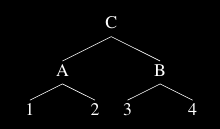
\includegraphics[width=0.3\textwidth]{tree}
    \end{center}
\end{figure}
where $A$ represents the winner of the match between competitors 1 and 2, $B$ represents the winner of
the match between competitors 3 and 4, and $C$ represents the winner of the match between $A$ and
$B$. The winner of this tourney is $C$.

Because of sponsorship contracts, some competitors will be replaced over time. After any new person
comes in, a new tourney is held.

In order to help Don Cherry, you must write a program to compute certain tourney statistics at
various points in time, given a sequence of $M$ $(1 \le M \le 1\,000\,000)$ commands -- see the input
format below.

\section*{Input}
The first line of input contains two integers, $N$ $(1 \le N \le 20)$ and $M$ $(1 \le M \le
1\,000\,000)$, separated by one space.

The next $2^N$ lines, for $i$ from $1$ to $2^N$, each contain one integer $S_i$, indicating the
skill level of the initial competitor at position $i$ in the tourney tree.

Each of the following M lines will be a command in one of three formats:
\begin{itemize}
\item ``R $i$ $S$'' means that the competitor at position $i$ is removed, and replaced with a new
one with skill level $S$. A new tourney is then held.
\item ``W'' means that your program should determine who won the current tourney. Print out the
position $i$ (between 1 and $2^N$) of this competitor.
\item “S $i$” means that your program should print out the number of rounds that the competitor at
position $i$ won in the current tourney.
\end{itemize}

\section*{Output}
For each ``W'' or ``S $i$'' command in the input, print out the corresponding integer on a line by
itself.
